\documentclass{beamer}
\usepackage{tikz}
\usepackage[all]{xy}
\usepackage{amsmath,amssymb}
\usepackage{hyperref}
\usepackage{graphicx}
\usepackage{algorithmic}
\usepackage{multirow}
 
\DeclareMathOperator*{\argmin}{arg\,min}
\DeclareMathOperator*{\Lik}{Lik}
\DeclareMathOperator*{\PoissonLoss}{PoissonLoss}
\DeclareMathOperator*{\Peaks}{Peaks}
\DeclareMathOperator*{\Segments}{Segments}
\DeclareMathOperator*{\argmax}{arg\,max}
\DeclareMathOperator*{\maximize}{maximize}
\DeclareMathOperator*{\minimize}{minimize}
\newcommand{\sign}{\operatorname{sign}}
\newcommand{\RR}{\mathbb R}
\newcommand{\ZZ}{\mathbb Z}
\newcommand{\NN}{\mathbb N}
\newcommand{\z}{$z = 2, 4, 3, 5, 1$} 

\newcommand{\algo}[1]{\textcolor{#1}{#1}}
\definecolor{PDPA}{HTML}{66C2A5}
\definecolor{CDPA}{HTML}{FC8D62}
\definecolor{GPDPA}{HTML}{4D4D4D}

% Set transparency of non-highlighted sections in the table of
% contents slide.
\setbeamertemplate{section in toc shaded}[default][100]
\AtBeginSection[]
{
  \setbeamercolor{section in toc}{fg=red} 
  \setbeamercolor{section in toc shaded}{fg=black} 
  \begin{frame}
    \tableofcontents[currentsection]
  \end{frame}
}

\begin{document}

\title{Neural network architecture and learning}

\author{
  Toby Dylan Hocking\\
  toby.hocking@nau.edu\\
  toby.hocking@r-project.org\\
}

\maketitle


\section{Fully connected multi-layer Neural Networks}

\begin{frame}
  \frametitle{Supervised learning setup}
  \begin{itemize}
  \item Have an input $\mathbf x\in\mathbb R^d$ -- a vector of $d$
    real numbers.
  \item And an output $y$ (real number: regression, integer ID:
    classification, spam filtering, images of digits/clothing, etc).
  \item Want to learn a prediction function $f(\mathbf x) = y$ that
    will work on a new input.
  \item In a neural network (or multi-layer perceptron) with $L-1$
    hidden layers, the function $f$ is defined using composition of
    $L$ functions, $f(x)=f^{(L)}[\cdots f^{(1)}[x] ]\in\mathbb R$.
  \item Linear model is special case with $L=1$ function, 0 hidden
    layers.
  \item ``Deep'' learning means $L\geq 3$ functions, at least 2 hidden
    layers.
  \end{itemize}
\end{frame}

\begin{frame}
  \frametitle{Each function is matrix multiplication and activation}
  \begin{itemize}
  \item Prediction function $f(x)=f^{(L)}[\cdots f^{(1)}[x] ]\in\mathbb R$.
  \item Each function $l\in\{1,\dots, L\}$ is a matrix multiplication
    followed by an activation function:
    $f^{(l)}[z] = \sigma^{(l)}[ W^{(l)} z ]$ where
    $W^{(l)}\in\mathbb R^{u^{(l)}\times u^{(l-1)}}$ is a weight matrix
    to learn, and $z\in\mathbb R^{u^{(l-1)}}$ is the input vector to
    that layer.
  \item If the loss function is defined in terms of a real-valued
    predicted score (typical, like we did in linear models), then the
    last activation function is fixed to the identity
    $\sigma^{(L)}[z]=z$.
\item The other activation functions must be
non-linear, e.g. 
logistic/sigmoid $\sigma(z)=1/(1+\exp(-z))$ or rectified linear units (ReLU) 
$$
\sigma(z)=
\begin{cases}
  z & \text{ if } z>0,\\
  0 & \text{ else.}
\end{cases}
$$ 
\end{itemize}
\end{frame}

\begin{frame}
  \frametitle{Non-linear activation functions}
$
\sigma(z)=
\begin{cases}
  z & \text{ if } z>0,\\
  0 & \text{ else.}
\end{cases}
$
  \hskip 1in
  $\sigma(z)=1/(1+\exp(-z))$

  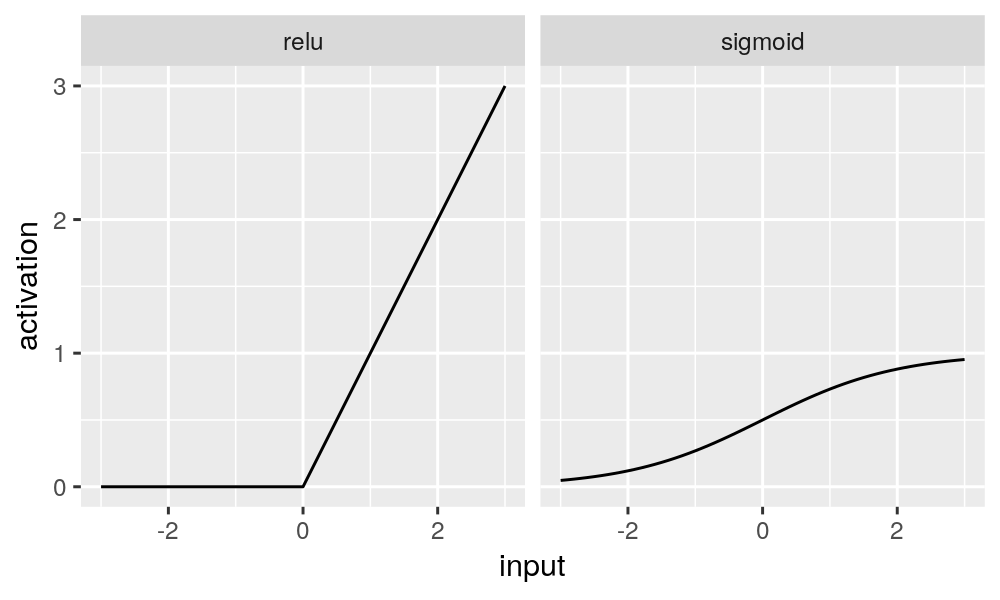
\includegraphics[width=\textwidth]{figure-activations}

\end{frame}

\begin{frame}
  \frametitle{Network size}
For binary classification
with inputs $x\in\mathbb R^d$, the overall neural network architecture
is $(u^{(0)}=d, u^{(1)}, \dots, u^{(L-1)}, u^{(L)}=1)$, where
$u^{(1)},\dots, u^{(L-1)}\in\mathbb Z_+$ are positive integers
(hyper-parameters that control the number of units in each hidden
layer, and the size of the parameter matrices $W^{(l)}$).
\begin{itemize}
\item ``Units'' is a synonym for ``features'' and ``variables.''
\item First and last layer are ``visible'' others are ``hidden.''
\item First layer size $u^{(0)}$ is fixed to input size.
\item Last layer size $u^{(L)}$ is fixed to output size.
\item Number of layers and hidden layer sizes
  $u^{(1)},\dots, u^{(L-1)}$ must be chosen (by you).
\item No hidden layers/units means $L=1$, linear model.
\item  ``Deep'' learning means $L\geq 3$ functions, at least 2 hidden
  layers.
\end{itemize}
\end{frame}

\begin{frame}
  \frametitle{Network diagram for linear model with 10 inputs/features}
  Neural network
  diagrams show how each unit (node) is computed by applying the
  weights (edges) to the values of the units at the previous layer.

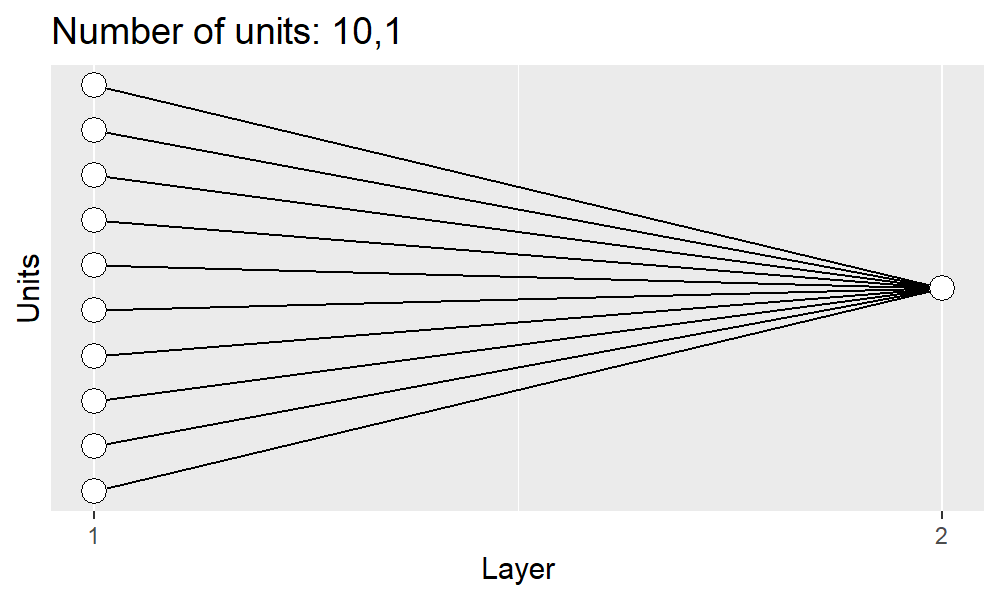
\includegraphics[width=\textwidth]{figure-architecture-linear}
\end{frame}

\begin{frame}
  \frametitle{Network diagram for single hidden layer with 2 units}
Neural network diagrams show how each unit (node) is computed by
applying the weights (edges) to the values of the units at the previous
layer.

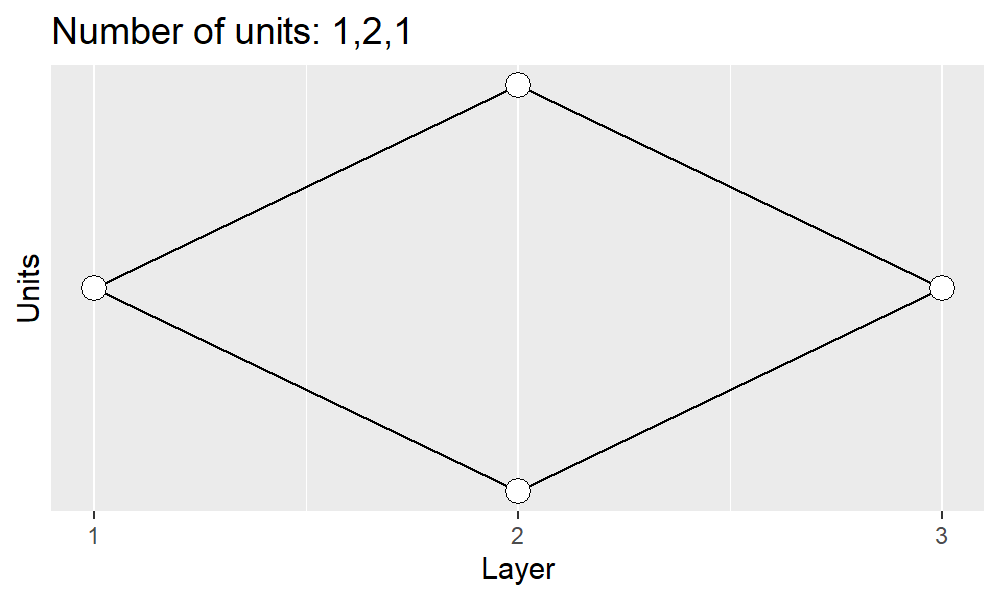
\includegraphics[width=\textwidth]{figure-architecture-reg2}
\end{frame}

\begin{frame}
  \frametitle{Network diagrams}
  Neural network
  diagrams show how each unit (node) is computed by applying the
  weights (edges) to the values of the units at the previous layer.

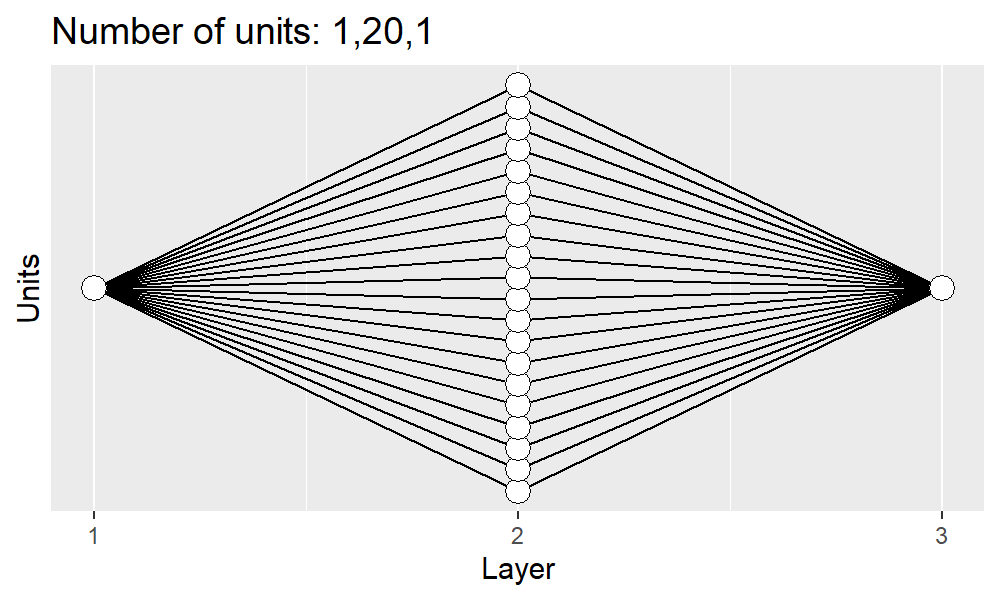
\includegraphics[width=\textwidth]{figure-architecture-reg20}
\end{frame}

\begin{frame}
  \frametitle{Network diagrams}
  Neural network
  diagrams show how each unit (node) is computed by applying the
  weights (edges) to the values of the units at the previous layer.

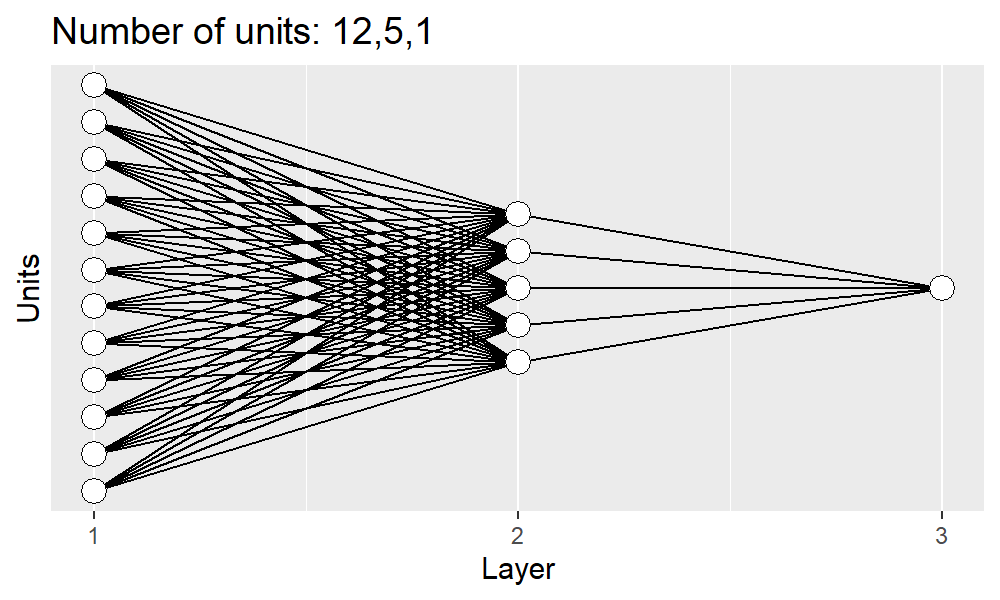
\includegraphics[width=\textwidth]{figure-architecture-oneOut}
\end{frame}

\begin{frame}
  \frametitle{Network diagrams}
  Neural network
  diagrams show how each unit (node) is computed by applying the
  weights (edges) to the values of the units at the previous layer.

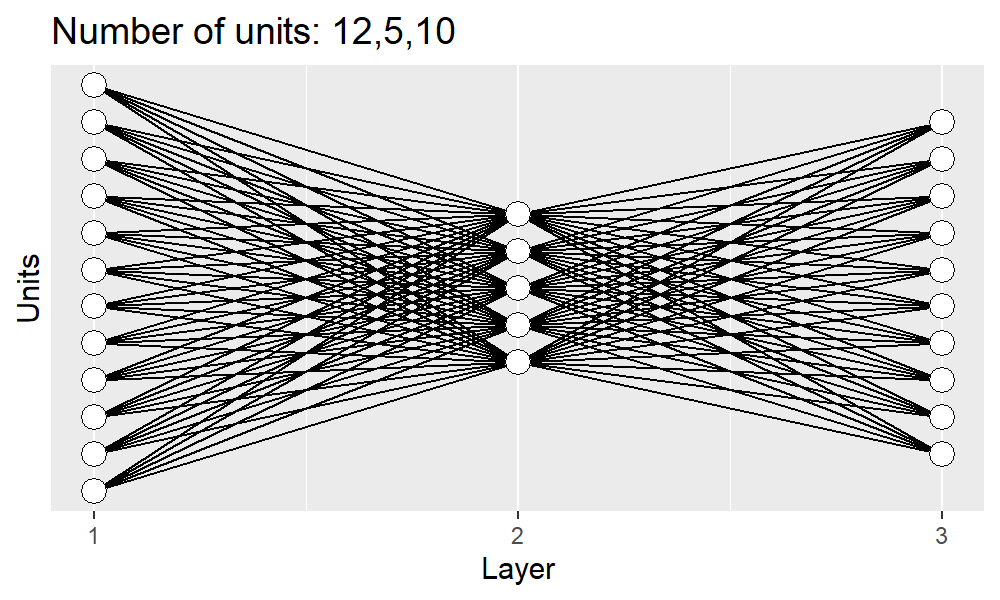
\includegraphics[width=\textwidth]{figure-architecture-tenOut}
\end{frame}

\begin{frame}
  \frametitle{Network diagrams}
  Neural network
  diagrams show how each unit (node) is computed by applying the
  weights (edges) to the values of the units at the previous layer.

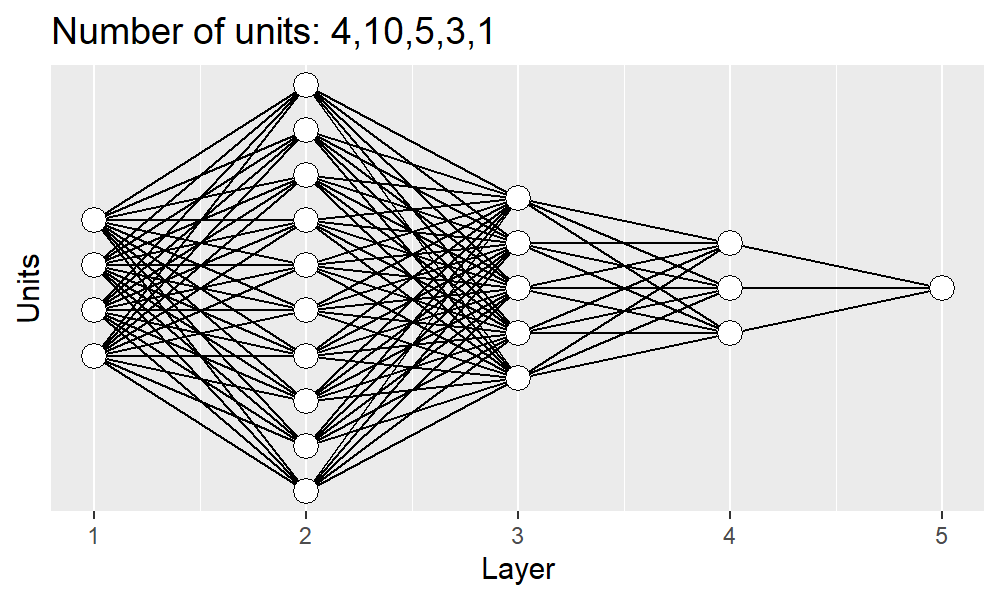
\includegraphics[width=\textwidth]{figure-architecture-fiveLayers}
\end{frame}

\begin{frame}
  \frametitle{Units in each layer}
We can write the units at each layer as
$h^{(0)},h^{(1)},\dots, h^{(L-1)}, h^{(L)}$ where
\begin{itemize}
\item $h^{(0)}=x\in\mathbb R^d$ is an input feature vector,
\item and
$h^{(L)}\in\mathbb R$ is the predicted output.
\end{itemize}
For
each layer $l\in \{1, \dots, L\}$ we have:
\begin{equation*}
  \label{eq:h_l}
  h^{(l)} = f^{(l)}\left[h^{(l-1)}\right] =
  \sigma^{(l)}\left[ W^{(l)} h^{(l-1)} \right].
\end{equation*}
Total number of parameters to learn is
$\sum_{l=1}^L u^{(l)} u^{(l-1)}.$

Quiz: how many parameters in a
neural network for $d=10$ inputs/features with one hidden layer with
$u=100$ units? (one output unit, ten output units)
\end{frame}

\section{Computing gradients and learning weights}

\begin{frame}
  \frametitle{Gradient descent learning}
  Basic idea of gradient descent learning algorithm is to iteratively
  update weights $\mathbf W = [W^{(1)}, \dots, W^{(L)} ]$ to improve
  predictions on the subtrain set.
  \begin{itemize}
  \item Need to define a loss function
    $\mathcal L(\mathbf W)$ which is differentiable, and
    takes small values for good predictions.
  \item Typically for regression we use the mean squared error, and
    for binary classification we use the mean logistic
    loss (sometimes called cross entropy).
  \item The mean loss $\mathcal L(\mathbf W)$ is averaged over all $N$
    observations or batches $i$:
    $$
    \mathcal L(\mathbf W) =
    \frac 1 N \sum_{i=1}^N
    \mathcal L(\mathbf W, \mathbf X_i, \mathbf y_i)
    $$
  \item The mean full gradient $\nabla \mathcal L(\mathbf W)$ is a function
    which tells us the local direction where the loss is most
    increasing:
    $$
    \nabla \mathcal L(\mathbf W) =
    \frac 1 N \sum_{i=1}^N
    \nabla \mathcal L(\mathbf W, \mathbf X_i, \mathbf y_i)
    $$
  \end{itemize}
\end{frame}

\begin{frame}
  \frametitle{Loss functions}
  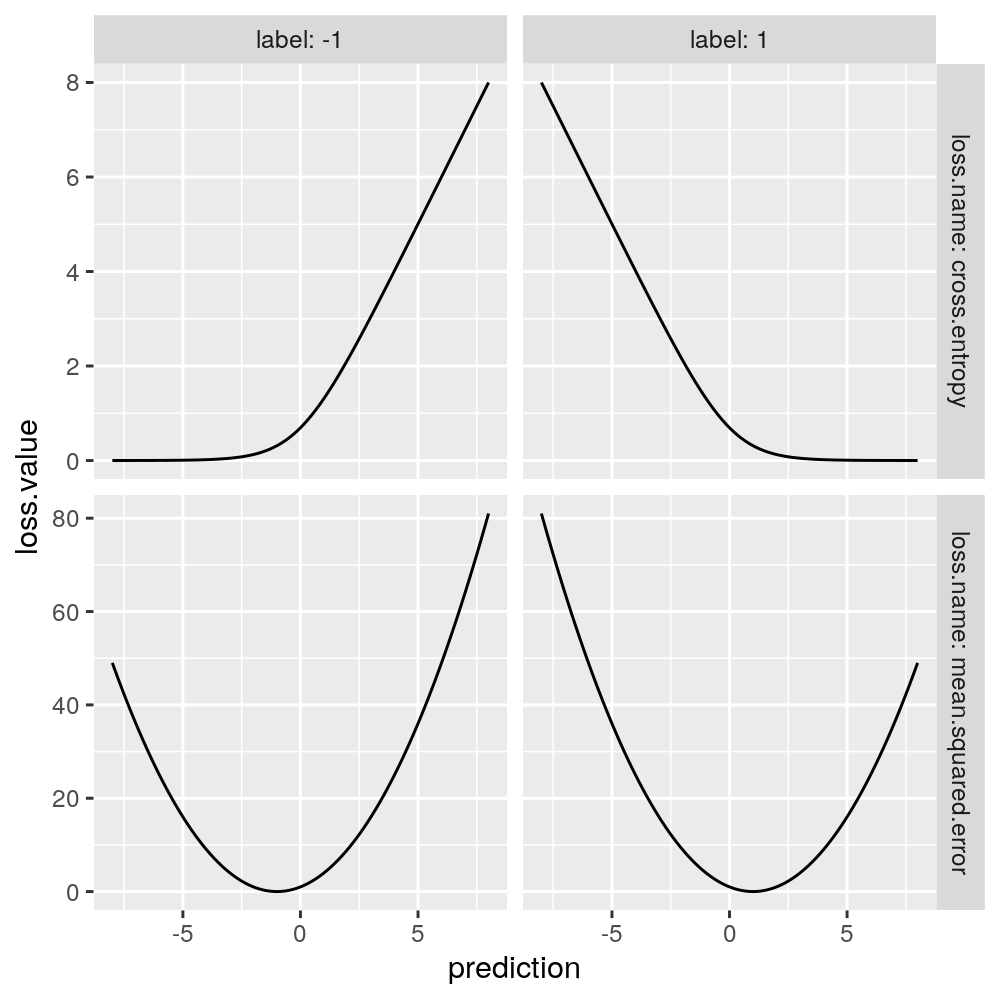
\includegraphics[width=0.8\textwidth]{figure-loss} 
\end{frame}

\begin{frame}
  \frametitle{Gradient descent animations}
  \url{https://yihui.org/animation/example/grad-desc/}

  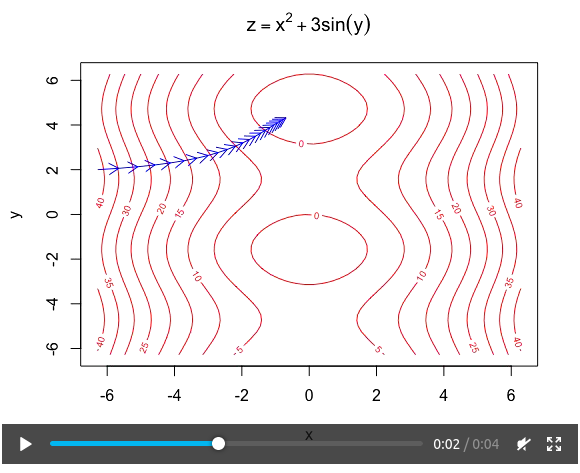
\includegraphics[width=0.9\textwidth]{screenshot-gradient-descent}
\end{frame}

\begin{frame}[fragile]
  \frametitle{Basic full gradient descent algorithm}
  \begin{itemize}
  \item Initialize weights $\mathbf W_0$ at some random values near
    zero (more complicated initializations possible).
  \item Since we want to decrease the loss, we take a step $\alpha>0$ in the
    opposite direction of the mean full gradient,
  $$
\mathbf W_t = \mathbf W_{t-1} - \alpha \nabla \mathcal L(\mathbf W_{t-1})
$$
\item This is the \textbf{full} gradient method (same as we did for
  linear models): batch size = $n$ =
  subtrain set size, so 1 step per epoch/iteration.
\end{itemize}

\end{frame}

\begin{frame}[fragile]
  \frametitle{Stochastic gradient descent algorithm}
  \begin{itemize}
  \item Initialize weights $\mathbf W$ at some random values near
    zero (more complicated initializations possible).
  \item for each epoch $t$ from 1 to max epochs:
  \item for each batch $i$ from 1 to $n$:
  \item Let $\mathcal L( \mathbf W, \mathbf X_i, \mathbf y_i )$ be the loss with
    respect to the single observation in batch $i$.
$$
\mathbf W \gets \mathbf W - \alpha \nabla \mathcal L(\mathbf W, \mathbf X_i, \mathbf y_i)
$$
\item This is the \textbf{stochastic} gradient method: batch size = 1,
  so there are $n$ steps per epoch.
\end{itemize}

\end{frame}

\begin{frame}[fragile]
  \frametitle{Batch (stochastic) gradient descent algorithm}
  \begin{itemize}
  \item Input: batch size $b$.
  \item Initialize weights $\mathbf W$ at some random values near
    zero (more complicated initializations possible).
  \item for each epoch $t$ from 1 to max epochs:
  \item for each batch $i$ from 1 to $\lceil n/b \rceil$:
  \item Let $\mathcal L( \mathbf W, \mathbf X_i, \mathbf y_i )$ be the
    mean loss with respect to the $b$ observations in batch $i$.
  $$
\mathbf W \gets \mathbf W - \alpha \nabla \mathcal L(\mathbf W, \mathbf X_i, \mathbf y_i)
$$
\item This is the \textbf{(mini)batch} stochastic gradient method:
  batch size = $b$, so there are $\lceil n/b \rceil$ steps per epoch.
\end{itemize}

\end{frame}

\begin{frame}[fragile]
  \frametitle{Forward propagation}
  \begin{itemize}
\item Forward propagation is the computation of hidden units
$h^{(1)},\dots,h^{(L)}$ given the inputs $x$ and current parameters
$W^{(1)},\dots,W^{(L)}$.
\item Start from input, apply weights and activation in each layer until
  predicted output is computed.
\item In the code this should be a for loop from first to last layer.
  \end{itemize}
\end{frame}

\begin{frame}[fragile]
  \frametitle{Back propagation}
Back propagation is the computation of gradients given current
parameters and hidden units.
\begin{itemize}
\item Start from loss function, compute gradient, send it to last
  layer, use chain rule, send gradient to previous layer, finally end
  up at first layer.
\item Result is gradients with respect to all weights in all layers.
\item Deep learning libraries like torch/keras do this using automatic
  differentiation based on your definition of the forward method and
  the loss function.
\item This week in class we will code the gradient computation from
  scratch to see how it works.
\item In the code this should be a for loop from last layer to first
  layer.
\end{itemize}


\end{frame}

\begin{frame}
  \frametitle{Computation graph}
  % from cs499-spring2020/notes.tex
  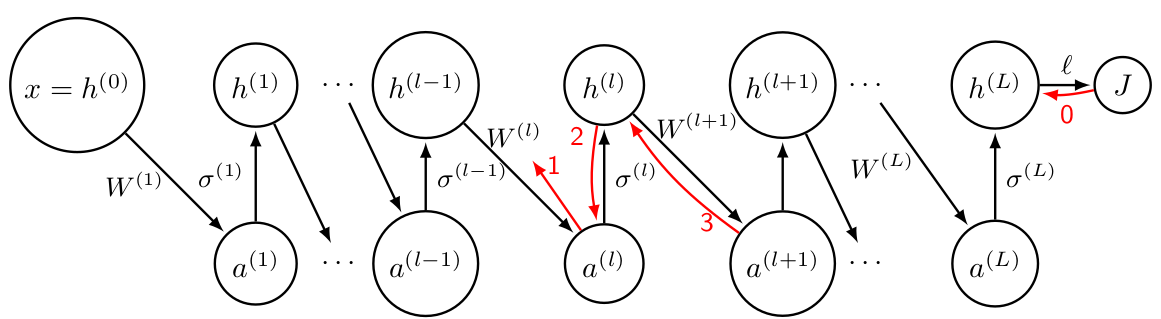
\includegraphics[width=\textwidth]{screenshot-backprop-figure}

For
each layer $l\in \{1, \dots, L\}$ we have:
\begin{eqnarray*}
  a^{(l)} &=&  W^{(l)} h^{(l-1)}, \\
  h^{(l)} &=& \sigma^{(l)}\left[ a^{(l)} \right].
\end{eqnarray*}
There are essentially four rules for computing gradients during
backpropagation (0-3).
  
\end{frame}

\begin{frame}
  \frametitle{Backprop rules}
  The rules 0--3 for backprop (from loss backwards):
\begin{description}
\item[Rule 0] computes $\nabla_{h^{(L)}} J$, which depends on the
  choice of the loss function $\ell$.
\item[Rule 1] computes
  $\nabla_{W^{(l)}} J$ using $\nabla_{a^{(l)}} J$, for any $l\in\{1,\dots,L\}$
\begin{eqnarray}
  \nabla_{W^{(l)}} J
  &=& \left( h^{(l-1)} \right)^T
      \left(\nabla_{a^{(l)}} J\right)
       \label{eq:grad-loss-w}
\end{eqnarray}
\item[Rule 2] computes
  $\nabla_{a^{(l)}} J$ using $\nabla_{h^{(l)}} J$, for any $l\in\{1,\dots,L\}$.
\begin{eqnarray}
  \nabla_{a^{(l)}} J
  &=& \left(\nabla_{h^{(l)}} J\right) \odot
      \label{eq:grad-loss-a}
      \left(\nabla_{a^{(l)}} h^{(l)} \right) 
  %&=& \left(\nabla_{h^{(l)}} J\right) \odot \left(h^{(l)}[1-h^{(l)}]\right).\label{eq:logistic-activation}
\end{eqnarray}
\item[Rule 3] computes
  $\nabla_{h^{(l)}} J$ using $\nabla_{a^{(l+1)}} J$, for any $l\in\{1,\dots,L-1\}$.
\begin{eqnarray}
  \nabla_{h^{(l)}} J
  &=& \left(\nabla_{a^{(l+1)}} J\right)
      \left(W^{(l+1)}\right)^T \label{eq:grad-loss-h}
\end{eqnarray}
\end{description}

\end{frame}

\begin{frame}
  \frametitle{Implementation details}
  \begin{itemize}
  \item Previous slides explained computations for a single
    observation, here we explain for a batch.
  \item Each $h^{(l)},a^{(l)}$ and their gradients can be stored as a
    matrix (nrow=batch size, ncol=$u^{(l)}$=number units in this layer).
  \item Each $W^{(l)}$ and its gradient is a $u^{(l-1)}\times u^{(l)}$
    matrix.
  \item You may want to code assertions to make sure each matrix is
    the correct shape.
  \item Matrix multiply features by weights to get next layer,
    $a^{(l)}=h^{(l-1)} W^{(l)}$.
  \item Use np.where to implement relu activation (output is
    non-negative).
  \item Make sure last activation is identity --- final predicted
    values should be real numbers (both positive and negative).
  \end{itemize}
\end{frame}


\begin{frame}
  \frametitle{Computation exercises (gradient descent learning)}
  Now assume we have used backpropagation to compute gradients with
  respect to four observations $i$:
  \begin{eqnarray*}
    \mathbf \nabla_{\mathbf v}
    \mathcal L(\mathbf v, \mathbf X_i,\mathbf y_i)
    &=& \begin{cases}
      [-1, 1] & i=1\\
      [-2, 2] & i=2\\
      [-3, 2] & i=3\\
      [-1, 2] & i=4
    \end{cases} 
  \end{eqnarray*}
  Starting at current weights $\mathbf v=[-2, 1]$ and using gradient descent
  with step size $\alpha=0.5$,   ($\mathcal L$ is total loss, show your work!)

  \begin{enumerate}
  \item For the full gradient method, there is one step. What is the
    new weight vector $\mathbf v$ after that step?
  \item For a batch size of 2, there are two steps. Assume batch 1 is
    observations $i=1,2$ and batch 2 is observations $i=3,4$. What is the new
    weight vector $\mathbf v$ after the batch 1 step? After the batch
    2 step?
  \item For the stochastic gradient method, there are four steps
    $i=1,2,3,4$. What is $\mathbf v$ after each
    of those steps?
  \end{enumerate}
\end{frame}

\section{Automatic differentiation}

\begin{frame}
  \frametitle{Why automatic differentiation?}
  \begin{itemize}
  \item Also called ``auto-grad,'' short for automatic gradient.
  \item People who design new neural network architectures and loss
    functions (fit method of learner class) do not necessarily have
    the expertise to compute the gradients.
  \item Automatic differentiation allows ``separation of concerns.''
  \item People who know how to compute gradients can implement classes
    which encapsulate forward/backward computations for individual
    operations (matrix multiplication, log, exp, etc).
  \item Other people can use these classes to implement their neural
    network, without having to know about the details of the
    forward/backward computations (and no worries about coding
    buggy/incorrect gradients).
  \end{itemize}
\end{frame}

\begin{frame}
  \frametitle{Computation graph for multi-layer perceptron}
  \begin{itemize}
  \item Each node in the computation graph is a tensor (0d=scalar,
    1d=vector, 2d=matrix, etc).
  \item Each edge in the computation graph is an operation (with
    methods for forward/back-prop).
  \item Only three operations needed: matrix multiply (\texttt{mm}),
    non-linear activation (\texttt{act}), and computing \texttt{loss} given
    labels $y$ and predicted scores $a^{(L)}$.
  \end{itemize}

  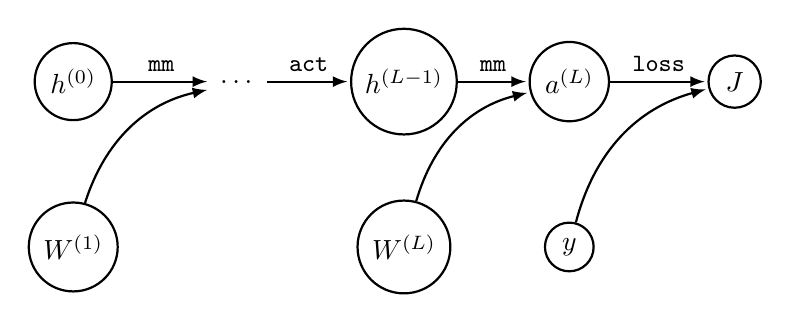
\begin{tikzpicture}[->,>=latex,shorten >=1pt,auto,node distance=2.1cm,
      thick,main node/.style={circle,draw}]
    \node[main node] (h0) {$h^{(0)}$};
    \node[main node] (W1) [below of=h0] {$W^{(1)}$};
    \node (dots) [right of=h0] {$\dots$};
    \node[main node] (hLm1) [right of=dots] {$h^{(L-1)}$};
    \node[main node] (WL) [below of=hLm1] {$W^{(L)}$};
    \node[main node] (aL) [right of=hLm1] {$a^{(L)}$};
    \node[main node] (y) [below of=aL] {$y$};
    \node[main node] (J) [right of=aL] {$J$};
    \path[every node/.style={font=\sffamily\small}]
    (h0) edge node {\texttt{mm}} (dots)
    (W1) edge [bend left] (dots)
    (dots) edge node {\texttt{act}}  (hLm1)
    (hLm1) edge node {\texttt{mm}} (aL)
    (WL) edge [bend left] (aL)
    (y) edge [bend left] (J)
    (aL) edge node {\texttt{loss}} (J)
    ;
  \end{tikzpicture}

\end{frame}

\begin{frame}
  \frametitle{Nodes in the computation graph}
  \begin{itemize}
  \item Each node in the computation graph can be represented by an
    instance of a python class.
  \item \texttt{value} attribute is a numpy array, result of forward
    propagation, computed during instantiation.
  \item \texttt{grad} attribute is a numpy array of same size,
    gradient of loss with respect to this node, result of
    back-propagation. 
  \item Main idea is to link these instances together to form a
    computation graph and \texttt{value} (forward pass),
    then recursively compute \texttt{grad} (backward pass).
  \end{itemize}
\end{frame}

\begin{frame}
  \frametitle{Initial nodes in the computation graph}
  \begin{itemize}
  \item Initial node in the computation graph can be represented by an
    instance of \texttt{InitialNode} class.
  \item \texttt{value} attribute is a numpy array, 
    stored on instantiation.
  \item Main uses are wrapping training data and neural network
    weights: \texttt{InitialNode(weight\_mat)},
    \texttt{InitialNode(feature\_mat)},
    \texttt{InitialNode(label\_vec)}.
  \end{itemize}

  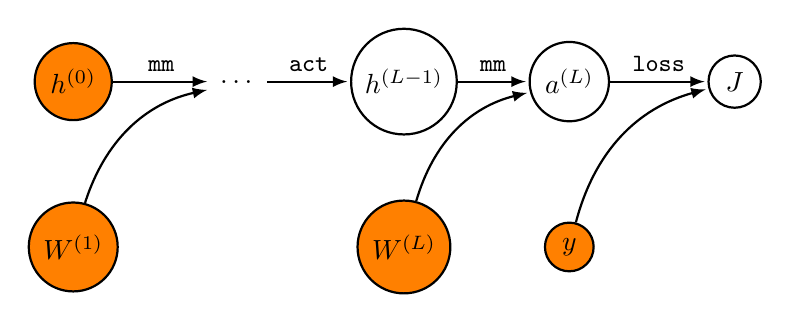
\begin{tikzpicture}[->,>=latex,shorten >=1pt,auto,node distance=2.1cm,
      thick,main node/.style={circle,draw}]
    \node[main node, fill=orange] (h0) {$h^{(0)}$};
    \node[main node, fill=orange] (W1) [below of=h0] {$W^{(1)}$};
    \node (dots) [right of=h0] {$\dots$};
    \node[main node] (hLm1) [right of=dots] {$h^{(L-1)}$};
    \node[main node, fill=orange] (WL) [below of=hLm1] {$W^{(L)}$};
    \node[main node] (aL) [right of=hLm1] {$a^{(L)}$};
    \node[main node, fill=orange] (y) [below of=aL] {$y$};
    \node[main node] (J) [right of=aL] {$J$};
    \path[every node/.style={font=\sffamily\small}]
    (h0) edge node {\texttt{mm}} (dots)
    (W1) edge [bend left] (dots)
    (dots) edge node {\texttt{act}}  (hLm1)
    (hLm1) edge node {\texttt{mm}} (aL)
    (WL) edge [bend left] (aL)
    (y) edge [bend left] (J)
    (aL) edge node {\texttt{loss}} (J)
    ;
  \end{tikzpicture}

\end{frame}

\begin{frame}
  \frametitle{Derived nodes in the computation graph}
  \begin{itemize}
  \item \texttt{Operation} class represents a node in the computation
    graph which is computed using other nodes.
  \item On instantiation, stores input nodes and does forward
    propagation.
  \item Method backward() computes gradient and recursively calls
    backward() on input nodes.
  \item \texttt{Operation} is virtual so we only instantiate sub-classes:
    \texttt{mm(features, weights)},
    \texttt{relu(a\_mat)},
    \texttt{logistic\_loss(a\_mat, label\_vec)}.
  \item Sub-classes should define \texttt{forward} and
    \texttt{gradient} methods which implement details of
    forward/back-prop, results are stored as \texttt{value}/\texttt{grad}
    attributes.
  \end{itemize}
\end{frame}

\begin{frame}
  \frametitle{Functions and gradients}
  \begin{itemize}
  \item $J = \text{logistic\_loss}(A, y)\in\mathbb R^{b\times 1}$ is
    same as in linear models. Values are
    $J_i = \log[1+\exp(-y_i A_i)]$ and gradient is
    $(\nabla_A J)_i = -y_i/(1+\exp(y_i A_i))$.
  \item $A = \texttt{mm}(X, W) = XW \in\mathbb R^{b\times u}$ where
    $X$ is a $b \times p$ matrix ($b=$number of samples in batch,
    $p=$number of units/features in this layer), and $W$ is a
    $p \times u$ matrix ($u=$number of units/features in next
    layer). Gradient of linear function is constant:
    $\nabla_X J = (\nabla_A J) (W^T)$,
    $\nabla_W J = X^T (\nabla_A J)$.
  \item $H = \texttt{relu}(A) \in\mathbb R^{b\times u}$ where each
    element $H_i = A_i\text{ if } A_i > 0\text{ else } 0$. Gradient
    $\nabla_A J = \nabla_A H \nabla_H J$ is piecewise constant, $(\nabla_A J)_i= (\nabla_H J)_i \text{ if } A_i > 0 \text{ else } 0$.
  \end{itemize}
  
\end{frame}

\begin{frame}
  \frametitle{Simple computation graph for linear model}
  \begin{itemize}
  \item Only two operations needed: matrix multiply (\texttt{mm}) and
    computing loss given predicted scores (\texttt{loss}).
  \item To implement the \texttt{loss} operation/class, you need to
    know how to compute the gradient of the loss (maybe difficult for
    complex loss functions).
  \end{itemize}

  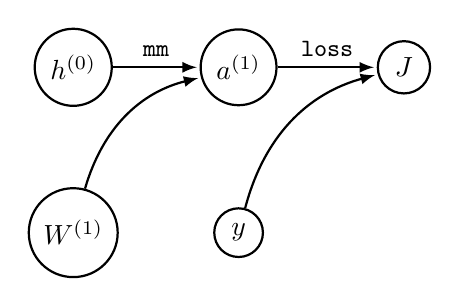
\begin{tikzpicture}[->,>=latex,shorten >=1pt,auto,node distance=2.1cm,
      thick,main node/.style={circle,draw}]
    \node[main node] (h0) {$h^{(0)}$};
    \node[main node] (W1) [below of=h0] {$W^{(1)}$};
    \node[main node] (a1) [right of=h0] {$a^{(1)}$};
    \node[main node] (y) [below of=a1] {$y$};
    \node[main node] (J) [right of=a1] {$J$};
    \path[every node/.style={font=\sffamily\small}]
    (h0) edge node {\texttt{mm}} (a1)
    (W1) edge [bend left] (a1)
    (y) edge [bend left] (J)
    (a1) edge node {\texttt{loss}} (J)
    ;
  \end{tikzpicture}

\end{frame}

\begin{frame}
  \frametitle{Detailed computation graph for linear model}
  \begin{itemize}
  \item Example: square loss $\ell(a^{(1)}, y) = (a^{(1)}-y)^2 = d^2$,
  \item Mean squared error: $J = \sum_{i=1}^n \ell(a_i^{(1)}, y_i)/n=\sum_{i=1}^n s_i/n$.
  \item More operations needed: matrix multiply (\texttt{mm}),
    subtraction (\texttt{diff}), \texttt{square}, \texttt{mean}.
  \item Each operation has a simple gradient (demo).
  \end{itemize}

  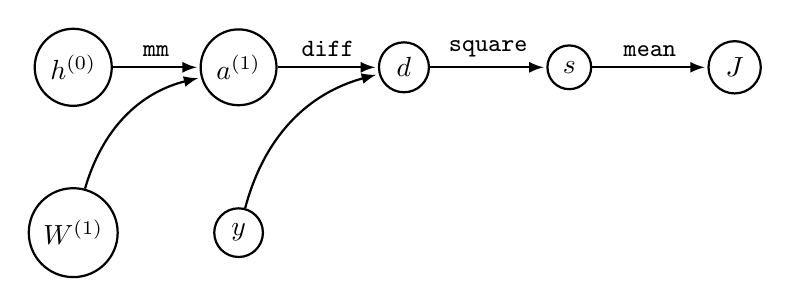
\begin{tikzpicture}[->,>=latex,shorten >=1pt,auto,node distance=2.1cm,
      thick,main node/.style={circle,draw}]
    \node[main node] (h0) {$h^{(0)}$};
    \node[main node] (W1) [below of=h0] {$W^{(1)}$};
    \node[main node] (a1) [right of=h0] {$a^{(1)}$};
    \node[main node] (y) [below of=a1] {$y$};
    \node[main node] (d) [right of=a1] {$d$};
    \node[main node] (s) [right of=d] {$s$};
    \node[main node] (J) [right of=s] {$J$};
    \path[every node/.style={font=\sffamily\small}]
    (h0) edge node {\texttt{mm}} (a1)
    (W1) edge [bend left] (a1)
    (y) edge [bend left] (d)
    (a1) edge node {\texttt{diff}} (d)
    (d) edge node {\texttt{square}} (s)
    (s) edge node {\texttt{mean}} (J)
    ;
  \end{tikzpicture}

\end{frame}

\begin{frame}
  \frametitle{Possible exam questions}
  \begin{itemize}
  \item Given a computation graph, and values for initial nodes,
    compute \texttt{value} in each derived node by hand (forward
    propagation), then compute \texttt{grad} (back-prop).
  \item In linear models we used scaling inside of the fit method ---
    make sure each feature/column has mean=0 and sd=1 before running
    gradient descent. What would you have to change in your neural
    network class to use scaling?
  \item In linear models we used gradient descent to learn an
    intercept parameter (a constant added to each real-valued
    prediction). We discussed two methods: (1) adding a column of ones
    to the feature matrix and an entry to the weight vector, or (2)
    adding a separate node representing the intercept in the
    computation graph. How would you modify your neural network class,
    using each method? (each hidden/output unit/feature in the neural
    network should have its own intercept parameter)
  \end{itemize}
\end{frame}

\section{Torch}

\begin{frame}
  \frametitle{torch}
  \begin{itemize}
  \item Machine learning library/module for python (and R, C++).
  \item Lots of standard neural network architectures and loss
    functions supported out of the box.
  \item Supports automatic differentiation! (easy to experiment with
    new models and loss functions without having to worry about
    gradient computations)
  \end{itemize}
\end{frame}

\begin{frame}[fragile]
  \frametitle{torch code for linear model for binary classification}
\begin{verbatim}
import torch
class LinearModel(torch.nn.Module):
    def __init__(self):
        super(LinearModel, self).__init__()
        self.weight_vec = torch.nn.Linear(n_features, 1)
    def forward(self, features):
        return self.weight_vec(features)
\end{verbatim}

  \begin{itemize}
  \item Linear is a matrix multiplication, with optional intercept
    (present by default, bias=False to suppress).
  \item One output because we are doing binary classification (want to
    predict a single real-valued score).
  \item Linear and other objects with weight parameters to learn must
    be assigned to an attribute of self (so torch.optim algorithms can
    find weights to update).
  \end{itemize}
\end{frame}

\begin{frame}[fragile]
  \frametitle{torch code for neural network with one hidden layer}
\begin{verbatim}
class OneHiddenLayer(torch.nn.Module):
    def __init__(self, n_features, n_hidden):
        super(Net, self).__init__()
        self.hidden_weights = torch.nn.Linear(
          n_features, n_hidden)
        self.activation = torch.nn.ReLU()
        self.out_weights = torch.nn.Linear(n_hidden, 1)
    def forward(self, feature_mat):
        a_mat = self.hidden_weights(feature_mat)
        h_mat = self.activation(a_mat)
        return self.out_weights(h_mat)
\end{verbatim}

Use activation after each Linear layer except for last.
\end{frame}

\begin{frame}[fragile]
  \frametitle{torch code for stack of hidden layers}
\begin{verbatim}
class Net(torch.nn.Module):
    def __init__(self, n_features, n_hidden):
        super(Net, self).__init__()
        self.stack = torch.nn.Sequential(
          torch.nn.Linear(n_features, n_hidden),
          torch.nn.ReLU(),
          torch.nn.Linear(n_hidden, 1))
    def forward(self, feature_mat):
        return self.stack(feature_mat)
\end{verbatim}
\end{frame}

\begin{frame}[fragile]
  \frametitle{Differences between gradient descent algorithm variants}

\begin{verbatim}
net = Net()
loss_fun = torch.nn.CrossEntropy()
optimizer = torch.optim.SGD(net.parameters(), lr=0.03)

# to do in a loop:
optimizer.zero_grad()
loss_value = loss_fun(net(inputs), outputs) # last node
loss_value.backward() # auto grad
optimizer.step() # learning

# stochastic, batch, full gradient descent variants:
loss_one = loss_fun(
  net(one_input), one_output)
loss_batch = loss_fun(
  net(batch_inputs), batch_outputs)
loss_subtrain = loss_fun(
  net(subtrain_inputs), subtrain_outputs)
\end{verbatim}

\end{frame}

\begin{frame}[fragile]
  \frametitle{Copy data from numpy and onto GPU}
  \begin{itemize}
  \item Torch is very similar to numpy (tensor data types, vectorized
    functions and methods).
  \item Can easily run on GPU for speedups, but need to copy neural network weights and data to GPU memory.
  \end{itemize}
\begin{verbatim}
device = "cuda" if torch.cuda.is_available() else "cpu"
# features and labels to torch and GPU
cpu_features = torch.from_numpy(numpy_features).float()
dev_features = cpu_features.to(device)
cpu_labels = torch.from_numpy(numpy_labels).float()
dev_labels = cpu_labels.to(device)
# weights to GPU
cpu_net = Net()
dev_net = cpu_net.to(device)
\end{verbatim}
\end{frame}

\begin{frame}[fragile]
  \frametitle{torch Dataset/DataLoader helpers for batching}
\begin{verbatim}
class CSV(torch.utils.data.Dataset):
    def __init__(self, features, labels):
        self.features = features
        self.labels = labels
    def __getitem__(self, item):
        return self.features[item,:], self.labels[item]
    def __len__(self):
        return len(self.labels)
ds = CSV(feature_mat, set_labels["subtrain"])
dl = torch.utils.data.DataLoader(
  ds, batch_size=1000, shuffle=True)
for batch_features, batch_labels in dl:
    # gradient descent code here.
\end{verbatim}

Not necessary (you can do your own batching), but can be useful.

\end{frame}


\end{document}